\documentclass[11pt]{article}
\usepackage[margin=1in]{geometry}
\usepackage{booktabs}
\usepackage{graphicx}
\usepackage{float}
\usepackage{amsmath}
\usepackage{array}
\usepackage{hyperref}
\usepackage[numbers]{natbib}
\usepackage[T1]{fontenc}
\usepackage{lmodern}

\title{Continuous-Time Graph Networks with Marked Point Processes for Asynchronous Market Microstructure}
\author{
Chetan Reddy Bojja\\
Georgia Institute of Technology\\
\texttt{cbojja3@gatech.edu}
}

\date{May 2026}

\graphicspath{{../figures/}{figures/}}

\begin{document}
\maketitle

\section*{Abstract}

This project looks at limit order book modeling from a more event-native point of view. Most standard LOB models first convert the book into fixed-time snapshots, but that process can easily lose some of the ordering and timing information which is naturally present in market data. The main idea here is that market microstructure is better treated as an asynchronous stream of marked events rather than as a regular image-like tensor.

I implemented a Continuous-Time Graph Neural Network (CT-GNN) with TGNMemory-style asynchronous memory updates, a marked next-event prediction objective and a full-book masked attention readout for short-horizon realized-volatility forecasting~\cite{rossi2020tgn,mei2017neuralhawkes}. The targets are computed from reconstructed mid-prices at 1s, 5s and 10s horizons. Evaluation is done with purged walk-forward splits and a five-minute embargo and the model is compared against timestamp-aligned DeepLOB and StaticGCN baselines.

On the canonical BTCUSDT 30-minute experiment, the CT-GNN restores positive all-event Spearman rank correlation across all three horizons. It also improves aligned rank-ordering compared with the neural discretized baselines. At the same time, the result is not a clean victory on RMSE or MAE and a simple Ridge baseline remains surprisingly strong. So the final claim is intentionally careful: the experiment gives evidence that event-native neural modeling can help with volatility rank forecasting under strict temporal controls, but it does not prove broad forecasting dominance.

\section{Introduction}

Limit order books do not move in neat, evenly spaced time steps. They evolve through irregular updates: limit order changes, cancellations, trades and depth movements that can arrive very quickly during active periods and much more slowly during quiet periods. A common approach in LOB forecasting is to force this stream into fixed-time snapshots, then train convolutional or graph-based models on those snapshots~\cite{zhang2019deeplob,ntakaris2018benchmark}.

That approach is convenient, but it also has a cost. Fixed-time sampling compresses the real event sequence. It can hide the order in which book changes happened, the time gaps between them and the causal structure of the market update process.

This project tries a different approach. Instead of treating the order book as a sequence of snapshots, I model it as a continuous event stream. Each event updates an asynchronous graph memory. Forecasts are made from the model state before the current event is used for memory updating, so the model cannot accidentally learn from the event it is being scored on. The model also jointly learns a next-event objective and a forward realized-volatility objective.

\section{Problem Motivation}

The main motivation for this work is temporal aliasing. When a high-frequency market is sampled at fixed intervals, the model sees a regular grid instead of the actual sequence of market events. In a busy market period, a single time bucket may contain many economically meaningful updates. In a quiet period, several buckets may contain almost no new information. These two situations look very different in the real market, but fixed snapshotting can blur the distinction.

A continuous-time model should be able to preserve more of this structure. It can keep track of event order, elapsed time, event type, side, level and location. This is especially relevant for short-horizon volatility forecasting, where the shape and speed of book updates can matter.

The target in this project is not directional return prediction. I focused on forward realized volatility over 1s, 5s and 10s horizons, computed from the reconstructed mid-price path. The central question is whether an event-native graph memory model can improve the rank-ordering of future volatility compared with fair discretized neural baselines.

\begin{figure}[H]
\centering
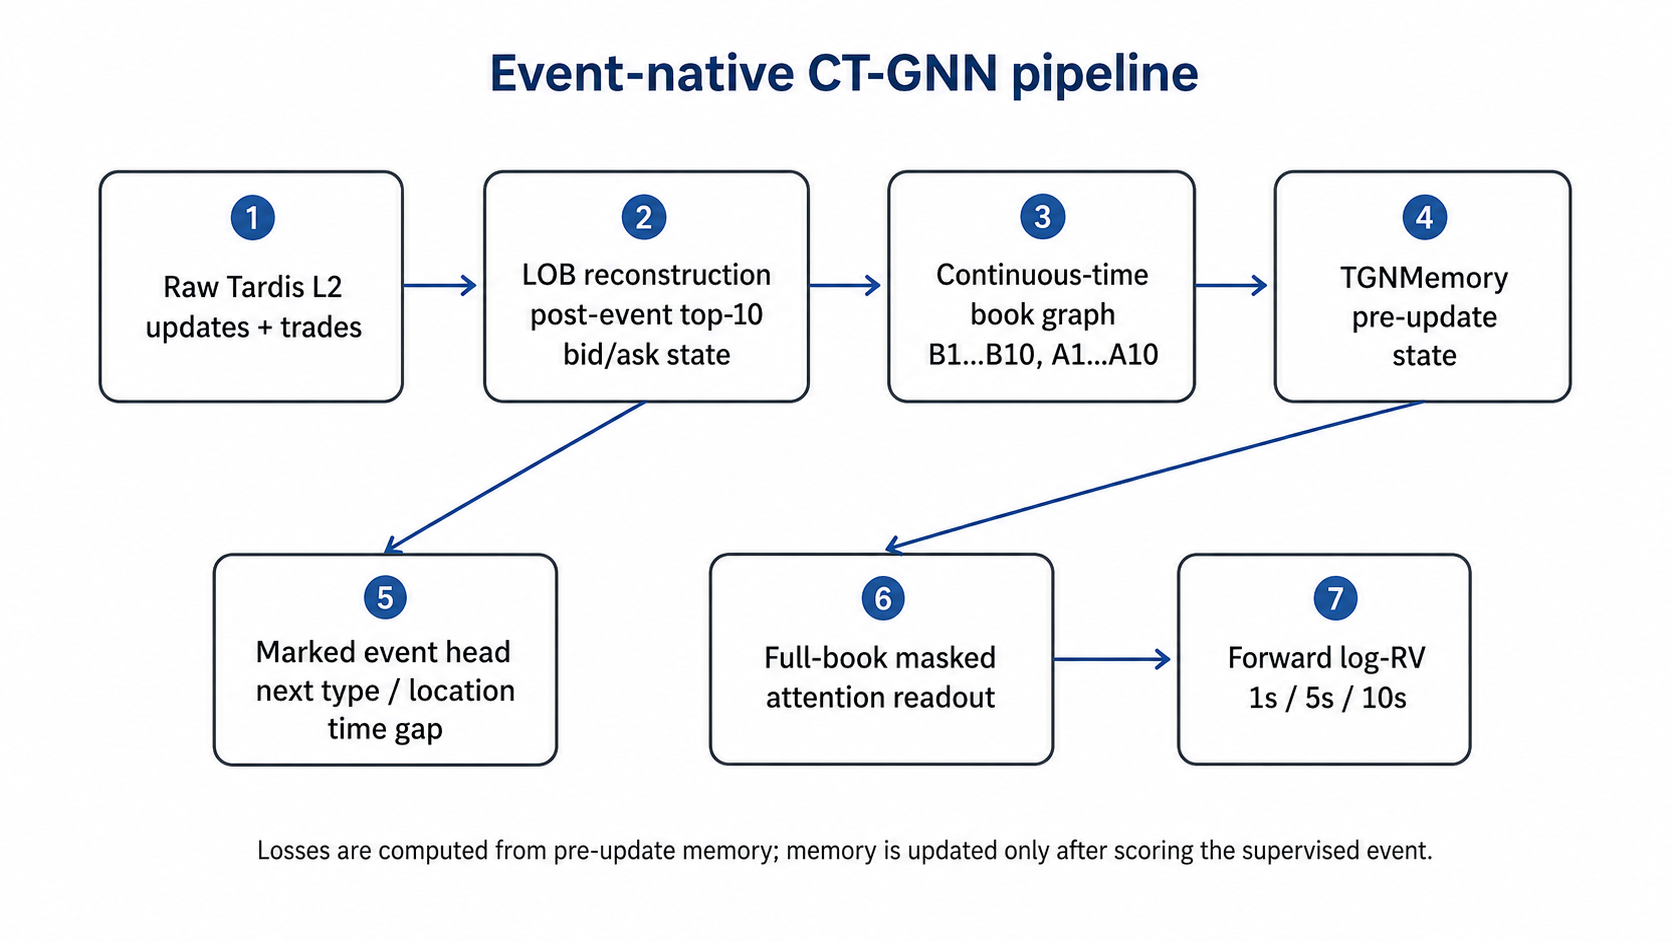
\includegraphics[width=0.98\textwidth]{fig_architecture_pipeline.png}
\caption{End-to-end event-native CT-GNN pipeline. Losses are computed from the pre-update memory state and the current event updates memory only after scoring.}
\label{fig:architecture}
\end{figure}
\newpage
\section{Data Reconstruction}

The canonical experiment uses Binance Futures BTCUSDT data from Tardis~\cite{tardisdocs}. The pipeline reads incremental L2 order book updates and trades, reconstructs the top-10 bid and ask book after each event and then writes event-level feature and target tables.

The protocol uses the following setup:

\begin{itemize}
  \item Symbol: BTCUSDT.
  \item Date: 2020-02-01.
  \item Trial window: 30 minutes.
  \item Reconstructed events after sanitation: 178,498.
  \item Visible book: 10 bid levels and 10 ask levels.
  \item Targets: real forward realized volatility from reconstructed mid-prices, not simulated depth or proxy price paths.
\end{itemize}

\begin{center}
\begin{tabular}{lr}
\toprule
Dataset / protocol quantity & Value \\
\midrule
Reconstructed events & 178,498 \\
Targets & 178,498 \\
Purged folds & 8 \\
Random seeds & 3 \\
DeepLOB aligned test samples & 5,476 \\
StaticGCN aligned test samples & 872 \\
Embargo length & 5 minutes \\
\bottomrule
\end{tabular}
\end{center}

The reconstruction audit confirms that the event-target join is one-to-one, timestamps are sorted, side/type/level/node values are valid, mid-prices are positive, spreads and sizes are non-negative and the full post-event LOB state columns are present.

\section{Model Architecture}

The CT-GNN represents the visible limit order book as graph nodes, with nodes corresponding to bid and ask price levels. The graph includes within-side level adjacency as well as cross-side same-distance structure. Each market event carries numeric microstructure features, side information, level information and event type information.

The model uses a TGNMemory-style asynchronous state~\cite{rossi2020tgn,pytorchgeometric}. Each event interacts with the graph memory and the memory is updated sequentially as the event stream progresses.

A key detail is the causal ordering. For each supervised event, the model first produces the prediction and computes the loss from the pre-update memory state. Only after that does the current event update memory. This prevents the model from using information from the same event before it is scored.

For volatility prediction, the model uses a masked full-book attention readout over populated visible nodes. This is useful because it lets the model aggregate information from the reconstructed book without treating missing levels as if they had real liquidity.

\section{Marked Event-Time Objective}

The model also includes a marked next-event objective~\cite{hawkes1971spectra,mei2017neuralhawkes}. The marked head predicts the next event type and next event location. The temporal part evaluates the observed time gap using a Monte Carlo intensity approximation.

The canonical run gives the following marked-event results:

\begin{center}
\begin{tabular}{lr}
\toprule
Metric & Value \\
\midrule
Next-event-type accuracy & $0.4962 \pm 0.0015$ \\
Next-location accuracy & $0.1202 \pm 0.0031$ \\
\bottomrule
\end{tabular}
\end{center}

I treat these numbers as supporting evidence that the model is learning nontrivial event-stream structure. However, the main claim of the project is still based on realized-volatility rank forecasting, not next-event prediction by itself.

\section{Experimental Protocol}

The final experiment is the canonical full-supervision CPU run:

\begin{verbatim}
python scripts/fetch_and_run_tardis_trial.py \\
  --date 2020-02-01 \\
  --trial-minutes 30 \\
  --train-minutes 10 \\
  --test-minutes 2 \\
  --embargo-minutes 5 \\
  --step-minutes 2 \\
  --min-train-events 2000 \\
  --min-test-events 500 \\
  --ctgnn-epochs 5 \\
  --baseline-epochs 4 \\
  --batch-size 32 \\
  --chunk-size 32 \\
  --seeds 42,43,44 \\
  --device cpu \\
  --no-train-on-spine \\
  --supervision-mode all_events
\end{verbatim}

The experiment uses 8 purged walk-forward folds, a five-minute embargo, three random seeds and full event supervision. The final result does not use supervised-spine acceleration.

The audit passed. The only warning is that saved node-populated mask columns were missing, so those masks were recomputed from bid and ask sizes.

\begin{figure}[H]
\centering
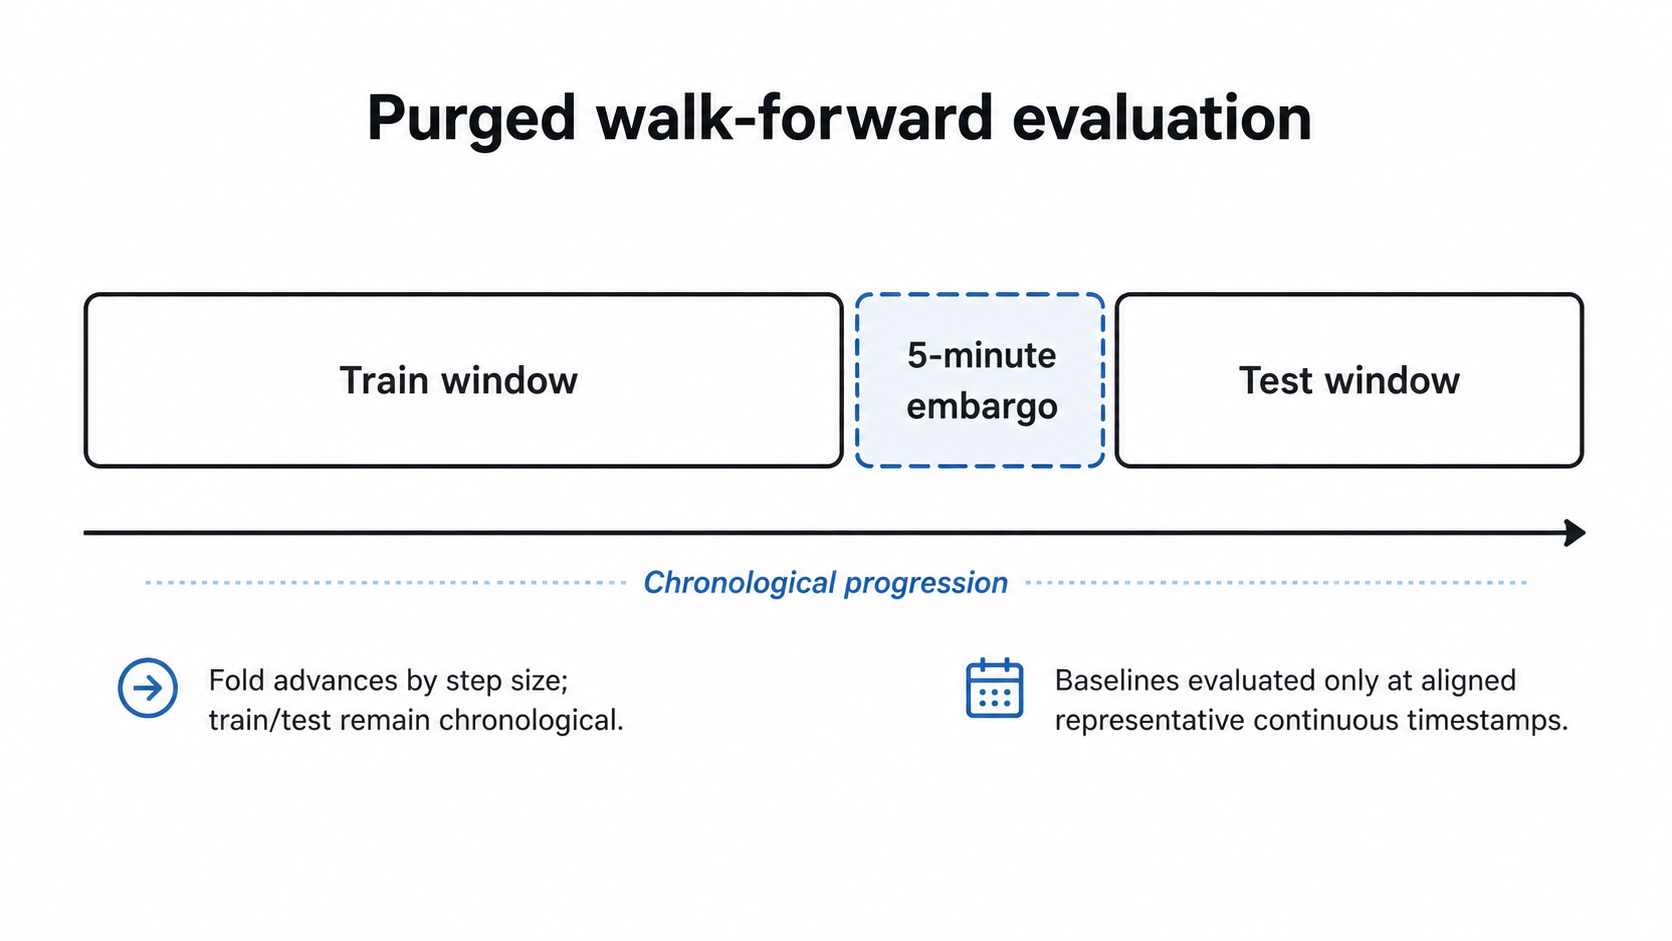
\includegraphics[width=0.95\textwidth]{fig_purged_walkforward.png}
\caption{Purged walk-forward evaluation. Each fold uses chronological train and test windows separated by a five-minute embargo. Discrete baselines are evaluated only at representative continuous event timestamps inside the same out-of-sample windows.}
\label{fig:purged_walkforward}
\end{figure}

\section{Baselines}

The neural baselines are DeepLOB and StaticGCN~\cite{zhang2019deeplob,kipf2017gcn}. DeepLOB is trained on fixed-time LOB tensors, while StaticGCN is trained on discrete graph snapshots. Both baselines inherit targets from representative continuous events and are evaluated only at aligned out-of-sample timestamps.

DeepLOB sequences are built within fold and split boundaries, so they do not cross purge regions. StaticGCN uses only the 20 visible bid and ask nodes.

I also include simpler baselines: persistence, rolling mean and Ridge regression on current-event and reconstructed-book features. Ridge is included only after a feature audit and negative-control checks.

\section{Results}

\subsection{CT-GNN All-Event Rank Forecasting}

On all CT-GNN test event times, the Spearman rank correlations are:

\begin{center}
\begin{tabular}{lr}
\toprule
Horizon & Spearman \\
\midrule
1s & $0.1041 \pm 0.0219$ \\
5s & $0.0785 \pm 0.1085$ \\
10s & $0.1883 \pm 0.0177$ \\
\bottomrule
\end{tabular}
\end{center}

The result is positive across all three horizons. The 10s horizon gives the strongest and most stable rank signal.

\begin{figure}[H]
\centering
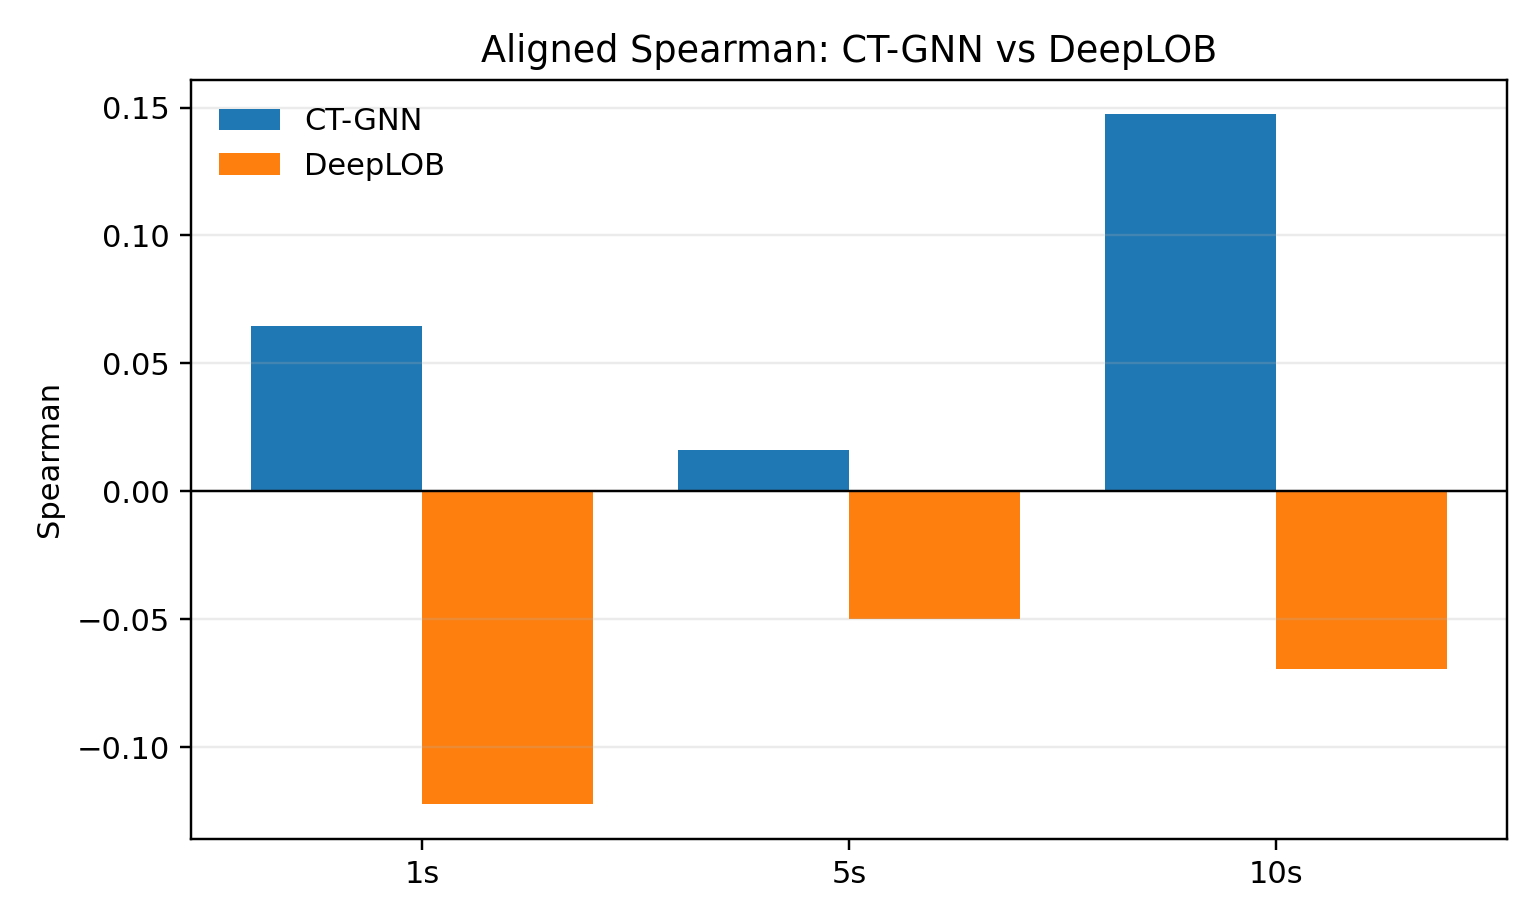
\includegraphics[width=0.82\textwidth]{fig_deeplob_spearman.png}
\caption{Aligned Spearman comparison between CT-GNN and DeepLOB. CT-GNN improves rank ordering at all three horizons on the DeepLOB-aligned out-of-sample timestamps.}
\label{fig:deeplob_spearman}
\end{figure}

\subsection{Aligned CT-GNN vs DeepLOB}

\begin{center}
\begin{tabular}{lrrr}
\toprule
Model & 1s & 5s & 10s \\
\midrule
CT-GNN & 0.0648 & 0.0162 & 0.1473 \\
DeepLOB & -0.1223 & -0.0500 & -0.0693 \\
\bottomrule
\end{tabular}
\end{center}

On the DeepLOB-aligned timestamps, CT-GNN has higher Spearman correlation at all three horizons.

\subsection{Aligned CT-GNN vs StaticGCN}

\begin{center}
\begin{tabular}{lrrr}
\toprule
Model & 1s & 5s & 10s \\
\midrule
CT-GNN & 0.0636 & -0.0720 & 0.0506 \\
StaticGCN & -0.0791 & -0.1434 & -0.2278 \\
\bottomrule
\end{tabular}
\end{center}

On the StaticGCN-aligned timestamps, CT-GNN again gives stronger Spearman rank correlation at every horizon. The 5s CT-GNN value is still negative, so this should not be overstated, but it remains less negative than the StaticGCN value.

\begin{figure}[H]
\centering
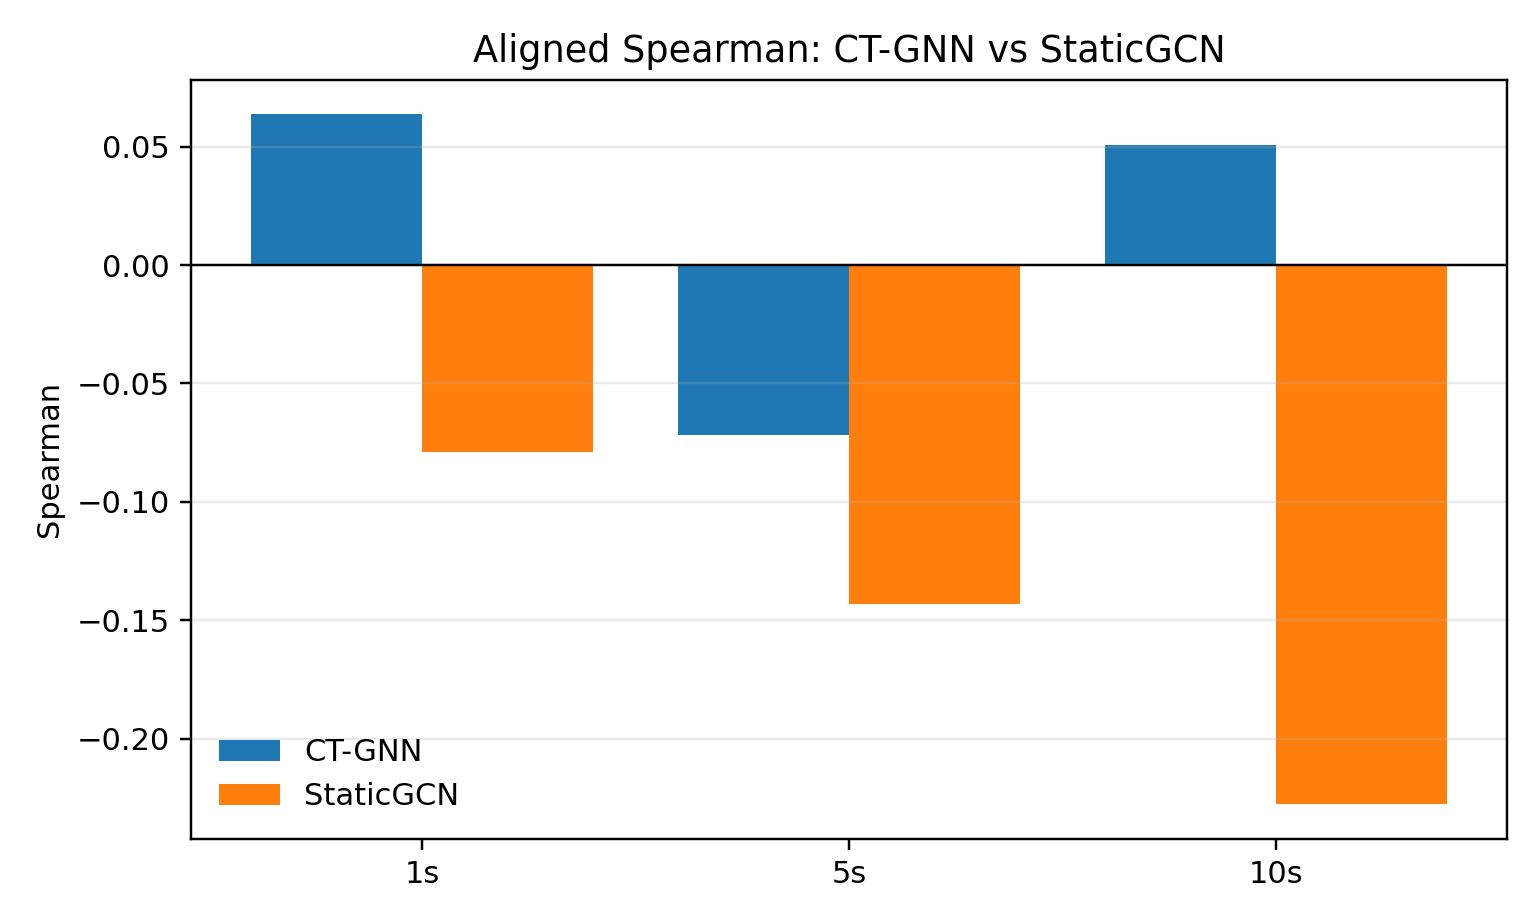
\includegraphics[width=0.82\textwidth]{fig_staticgcn_spearman.png}
\caption{Aligned Spearman comparison between CT-GNN and StaticGCN. CT-GNN is stronger on rank correlation, while StaticGCN remains competitive on point-error calibration.}
\label{fig:staticgcn_spearman}
\end{figure}

\subsection{Error Metrics}

The results are not a simple RMSE or MAE win for CT-GNN. DeepLOB and StaticGCN remain competitive and in several cases they perform better on absolute-error metrics. The fairest interpretation is that CT-GNN improves rank-ordering relative to the neural discretized baselines, but calibration and point-error prediction are still unresolved.

The full generated CSV files contain all RMSE and MAE values. The key neural-baseline RMSE comparison is:

\begin{center}
\begin{tabular}{llrrr}
\toprule
Aligned set & Model & RMSE 1s & RMSE 5s & RMSE 10s \\
\midrule
DeepLOB timestamps & CT-GNN & 6.0622 & 4.8098 & 3.9865 \\
DeepLOB timestamps & DeepLOB & 3.9400 & 4.0463 & 3.6862 \\
StaticGCN timestamps & CT-GNN & 6.4002 & 5.2283 & 4.3882 \\
StaticGCN timestamps & StaticGCN & 3.7376 & 4.2855 & 4.2408 \\
\bottomrule
\end{tabular}
\end{center}

\begin{figure}[H]
\centering
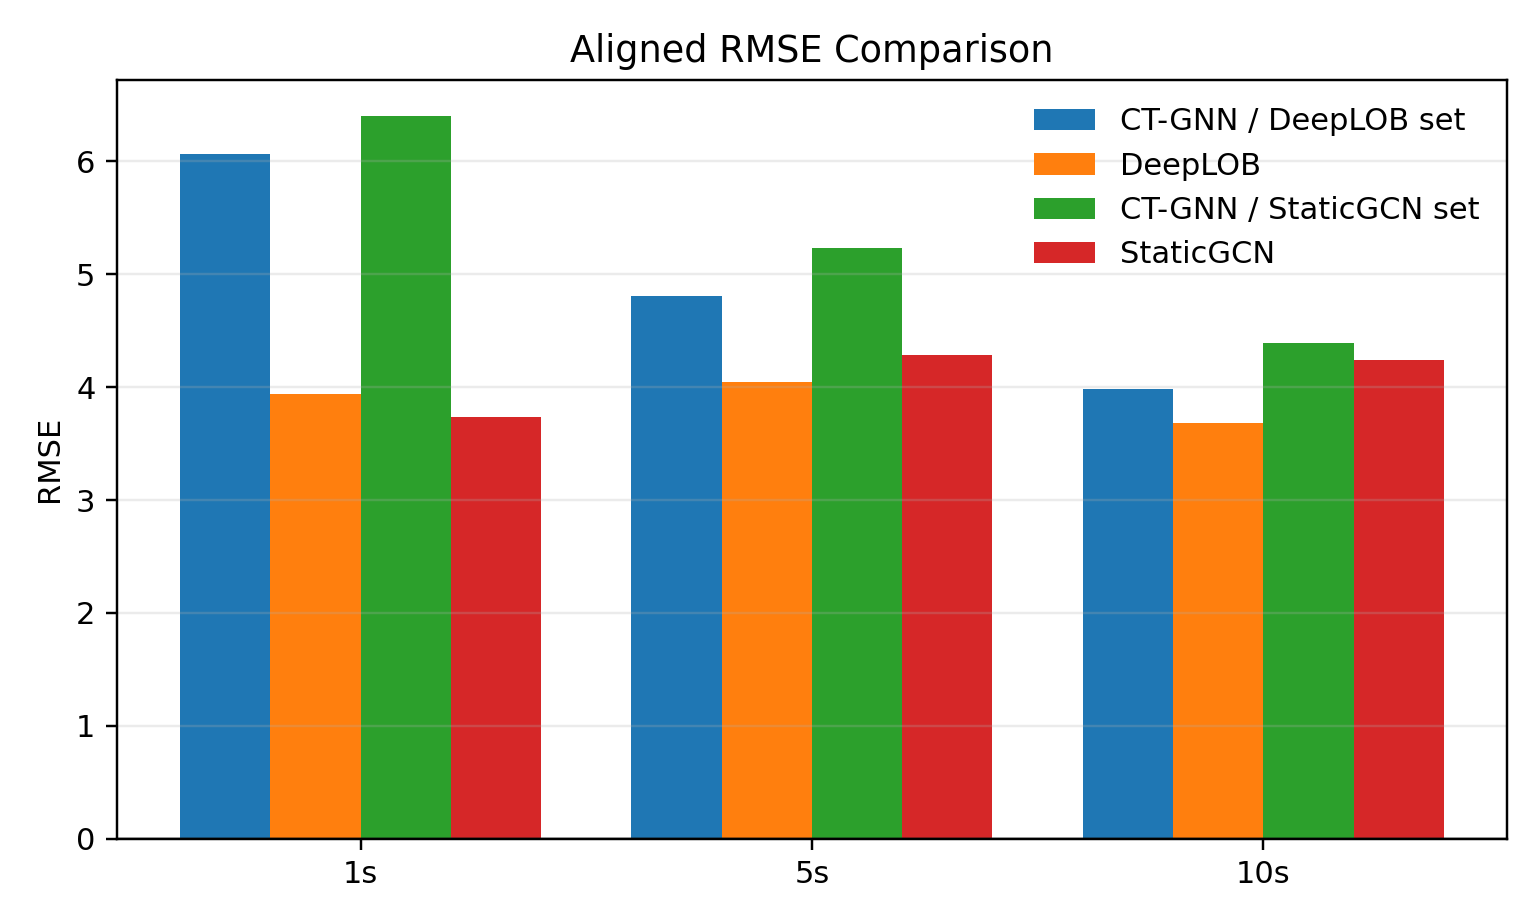
\includegraphics[width=0.82\textwidth]{fig_rmse_calibration.png}
\caption{Calibration view using 10s RMSE. CT-GNN's current strength is rank-ordering rather than point-error calibration.}
\label{fig:rmse_calibration}
\end{figure}

\section{Ridge Audit and Negative Controls}

Ridge regression turns out to be a surprisingly strong clean linear baseline~\cite{hastie2009elements}. The Ridge feature
records 49 current-event and reconstructed-book features per fold. It also checks that no target-derived or future-looking columns are used. In particular, it excludes \texttt{rv\_1s}, \texttt{rv\_5s}, \texttt{rv\_10s}, \texttt{log\_rv}, \texttt{future\_return}, \texttt{future\_mid}, \texttt{target\_end} and other horizon-derived columns. Feature scalers are fit only on the training portion of each fold.

The Ridge results and controls are:

\begin{center}
\begin{tabular}{lrrr}
\toprule
Model & 1s & 5s & 10s \\
\midrule
RidgeClean & 0.4935 & 0.2412 & 0.1674 \\
RidgeShuffledY & 0.0499 & 0.0378 & 0.0599 \\
RidgeTimestampPermuted & 0.0070 & -0.0012 & -0.0066 \\
\bottomrule
\end{tabular}
\end{center}

The timestamp-permutation control collapses close to zero, which makes trivial timestamp leakage less likely. The shuffled-target control is also much weaker than clean Ridge. Even with those checks, Ridge remains a major limitation and an important finding. In this short trial, the current LOB state contains strong linear information for ranking future volatility.

\begin{figure}[H]
\centering
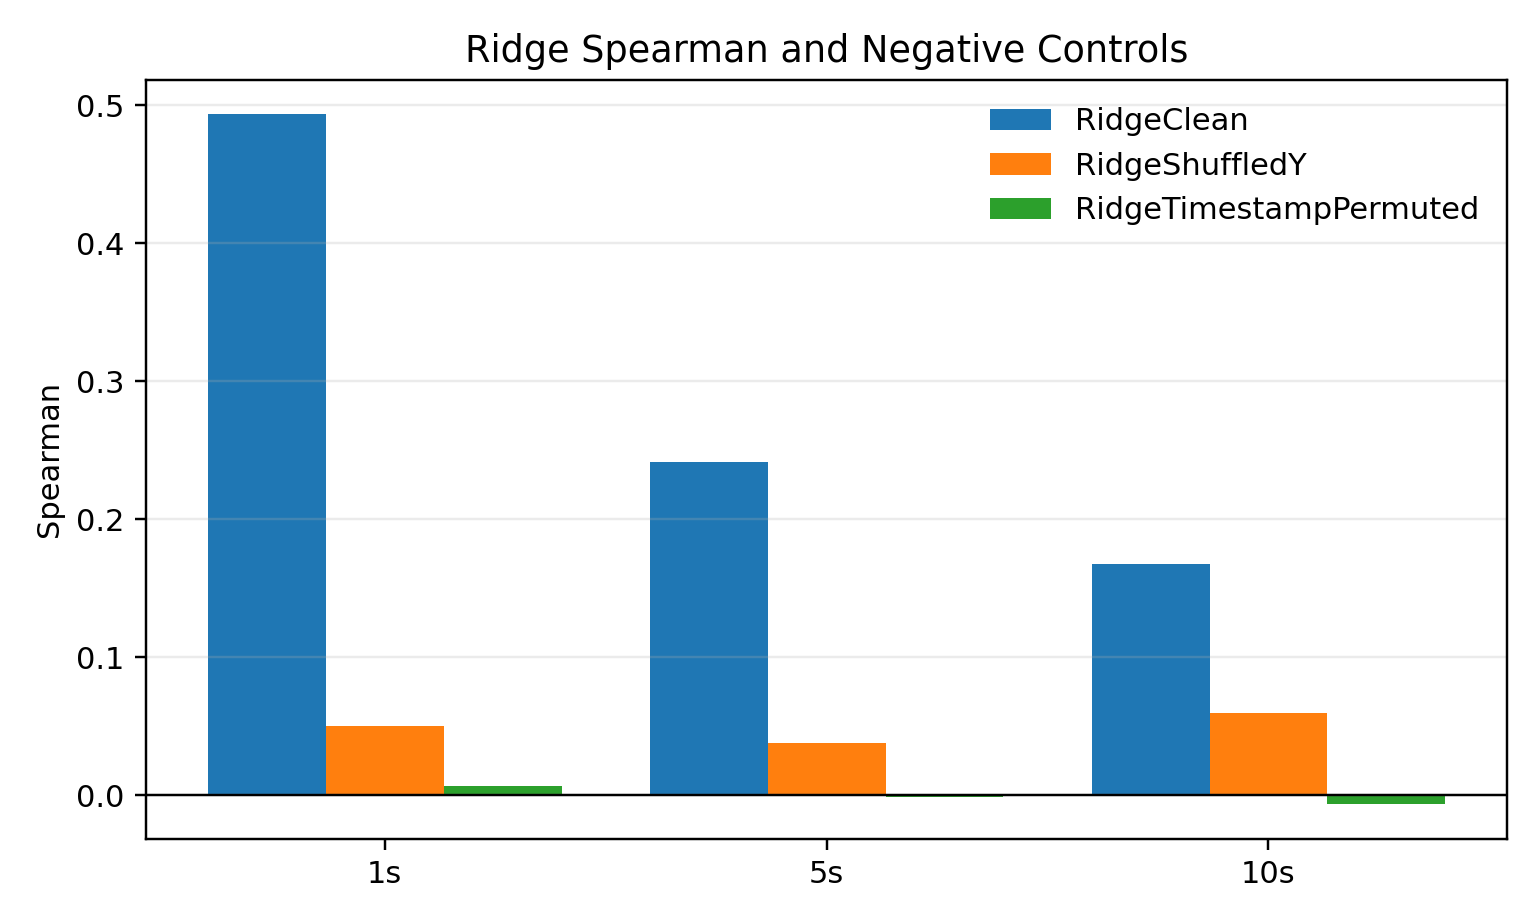
\includegraphics[width=0.86\textwidth]{fig_ridge_controls.png}
\caption{Ridge audit results. Clean Ridge is strong, while shuffled-target and timestamp-permutation controls collapse toward low or near-zero Spearman.}
\label{fig:ridge_controls}
\end{figure}

\section{Discussion}

The project builds a complete temporally controlled event-native research pipeline. The CT-GNN results support the idea that continuous-time graph memory can improve volatility rank-ordering compared with discretized neural baselines, at least under this strict aligned evaluation setup.

The strongest evidence comes from the aligned Spearman comparisons. CT-GNN outperforms both DeepLOB and StaticGCN on rank correlation across all reported aligned horizons. This suggests that preserving asynchronous event structure is useful for relative volatility forecasting.

A few important observations are that Ridge is stronger on few rank metrics and the neural baselines often do better on RMSE and MAE. The result says that the current CT-GNN is better at picking up relative volatility patterns than giving very exact calibrated values. It understands the event-level market structure well enough to rank future volatility and with some calibration, the log realized volatility magnitudes will become more accurate.




\section{Limitations}

\begin{itemize}
  \item Ridge is very strong and must remain a serious baseline in future work.
  \item CT-GNN does not dominate absolute-error metrics in every case.
  \item GPU was slower than CPU for this PyG and TGN memory-update workload due to serialization instead of parallelization.
  \item Full event supervision is computationally expensive because memory updates are sequential, but results in better output.
\end{itemize}

\section{Future Work}

Future work will experiment across more dates, symbols and market regimes. A year-scale CT-GNN run over every event is not practical with the current full-supervision implementation, because the memory updates are sequential and expensive.

A more scalable path would use a two-tier setup. First building daily feature-lake tables and evaluate Ridge, ElasticNet, LightGBM and other tabular models with rolling walk-forward validation. Second, run CT-GNN selectively on high-information windows, such as high-volatility periods, high event-intensity periods, liquidity-depletion regimes and intervals where cheaper baselines fail.

A scaled version will include a larger historical archive, statistical testing across days, improved calibration through target normalization and eventually cost-aware trading simulations. The current submission shows a controlled proof of the event-native framework.

\section{Conclusion}

This project delivers an end-to-end continuous-time LOB modeling pipeline with real data reconstruction, asynchronous graph memory, marked event-time modeling, full-book volatility readout, purged walk-forward evaluation, aligned neural baselines, simple baselines and Ridge leakage audits.

The result supports a measured conclusion: CT-GNN improves the rank-ordering of future realized volatility compared with neural discretized baselines under temporal evaluation. The main contribution is the event-native framework and the evaluation setup that will result in trading alpha during the discussed two-tier setup.

\appendix

\section{Reproducibility Artifacts}

The repository contains the final report, audit report, Ridge audit summary, run manifest, result tables and figures. The run manifest records the exact command-line arguments, CPU backend, PyTorch and PyG versions, reconstructed event count, fold count.


\section{Full Main Result Table}

\begin{center}
\begin{tabular}{llrrr}
\toprule
Model / evaluation set & Samples & Spearman 1s & Spearman 5s & Spearman 10s \\
\midrule
CT-GNN, all event times & 70,804 & 0.1041 & 0.0785 & 0.1883 \\
CT-GNN, DeepLOB-aligned & 5,476 & 0.0648 & 0.0162 & 0.1473 \\
DeepLOB & 5,476 & -0.1223 & -0.0500 & -0.0693 \\
CT-GNN, StaticGCN-aligned & 872 & 0.0636 & -0.0720 & 0.0506 \\
StaticGCN & 872 & -0.0791 & -0.1434 & -0.2278 \\
RidgeClean & -- & 0.4935 & 0.2412 & 0.1674 \\
RidgeShuffledY & -- & 0.0499 & 0.0378 & 0.0599 \\
RidgeTimestampPermuted & -- & 0.0070 & -0.0012 & -0.0066 \\
\bottomrule
\end{tabular}
\end{center}
\newpage













\begin{thebibliography}{9}

\bibitem{zhang2019deeplob}
Z. Zhang, S. Zohren, and S. Roberts.
\newblock DeepLOB: Deep convolutional neural networks for limit order books.
\newblock \emph{IEEE Transactions on Signal Processing}, 67(11):3001--3012, 2019.

\bibitem{ntakaris2018benchmark}
A. Ntakaris, M. Magris, J. Kanniainen, M. Gabbouj, and A. Iosifidis.
\newblock Benchmark dataset for mid-price forecasting of limit order book data with machine learning methods.
\newblock \emph{Journal of Forecasting}, 37(8):852--866, 2018.

\bibitem{rossi2020tgn}
E. Rossi, B. Chamberlain, F. Frasca, D. Eynard, F. Monti, and M. Bronstein.
\newblock Temporal graph networks for deep learning on dynamic graphs.
\newblock \emph{arXiv preprint arXiv:2006.10637}, 2020.

\bibitem{hawkes1971spectra}
A. G. Hawkes.
\newblock Spectra of some self-exciting and mutually exciting point processes.
\newblock \emph{Biometrika}, 58(1):83--90, 1971.

\bibitem{mei2017neuralhawkes}
H. Mei and J. Eisner.
\newblock The neural Hawkes process: A neurally self-modulating multivariate point process.
\newblock In \emph{Advances in Neural Information Processing Systems}, 2017.

\bibitem{tardisdocs}
Tardis.dev.
\newblock Historical cryptocurrency market data feeds and HTTP API documentation.
\newblock \url{https://docs.tardis.dev/api/http}.


\bibitem{pytorchgeometric}
M. Fey and J. E. Lenssen.
\newblock Fast graph representation learning with PyTorch Geometric.
\newblock \emph{arXiv preprint arXiv:1903.02428}, 2019.

\bibitem{hastie2009elements}
T. Hastie, R. Tibshirani, and J. Friedman.
\newblock \emph{The Elements of Statistical Learning}.
\newblock Springer, 2009.

\bibitem{kipf2017gcn}
T. N. Kipf and M. Welling.
\newblock Semi-supervised classification with graph convolutional networks.
\newblock In \emph{International Conference on Learning Representations}, 2017.

\end{thebibliography}
\end{document}
